\SourcePage{778}{781}
\renewcommand{\thesection}{\alph{section}}
\setcounter{section}{1}
\section{The Airy function}
\setcounter{figure}{53}

The equation
\begin{equation}
 y''-xy=0
 \tag{b.1}
\end{equation}
also belongs to the Laplace type. Following the general method, we form the
functions
\[
 P=t^2,\hspace{1.5em}Q=-1,\hspace{1.5em}
 Z=-\exp(-t^3/3),\hspace{1.5em}V=\exp(xt-t^3/3),
\]

\SourcePage{779}{782}
so that a solution can be represented as
\begin{equation}
 y(x)=\mathrm{const}\cdot\int_C\exp(xt-t^3/3)\,dt,
 \tag{b.2}
\end{equation}
where the integration path $C$ must be chosen so that $V$ vanishes at both
ends. For this purpose, the ends must tend to infinity in those regions of the
complex $t$ plane where $\operatorname{Re}(t^3)>0$ (these regions are shaded
in Fig.~54).

A solution finite for every $x$ is obtained by choosing $C$ as shown in the
figure. The path may be displaced arbitrarily, provided only that its ends go
to infinity in the same two shaded sectors ($I$ and $III$ in Fig.~54). Notice
that a path passing, for example, through sectors $III$ and $II$ would give a
solution tending to infinity as $x\to\infty$.

\begin{figure}[ht]
\centering
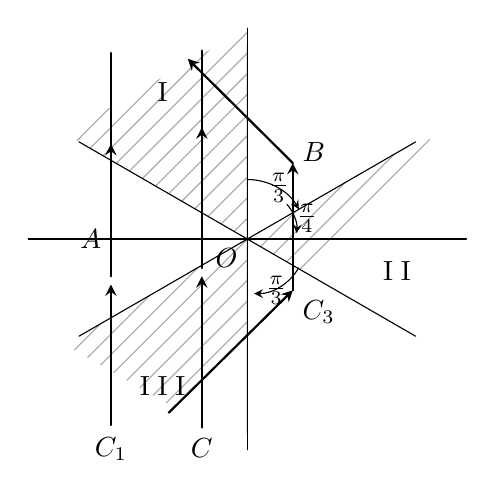
\begin{tikzpicture}[scale=1.05,>=stealth,line cap=round,line join=round]
  % The three sectors Re(t^3)>0.
  \begin{scope}
    \clip (0,0)--(90:2.55)--(150:2.55)--cycle;
    \foreach \k in {-4,-3.75,...,4}{\draw[gray!70,thin] (-3,\k)--(3,{\k+6});}
  \end{scope}
  \begin{scope}
    \clip (0,0)--(-30:2.55)--(30:2.55)--cycle;
    \foreach \k in {-4,-3.75,...,4}{\draw[gray!70,thin] (-3,\k)--(3,{\k+6});}
  \end{scope}
  \begin{scope}
    \clip (0,0)--(210:2.55)--(270:2.55)--cycle;
    \foreach \k in {-4,-3.75,...,4}{\draw[gray!70,thin] (-3,\k)--(3,{\k+6});}
  \end{scope}
  \draw[thin] (-2.65,0)--(2.65,0);
  \draw[thin] (0,-2.55)--(0,2.55);
  \draw[thin] (0,0)--(150:2.35) (0,0)--(90:2.35)
             (0,0)--(30:2.35) (0,0)--(-30:2.35)
             (0,0)--(210:2.35) (0,0)--(270:2.35);
  \node at (120:2.05) {$\mathrm I$};
  \node at (-12:1.85) {$\mathrm{I\;I}$};
  \node at (240:2.05) {$\mathrm{I\;I\;I}$};
  \node[below left] at (0,0) {$O$};
  % Paths C_1, C and C_3.
  \draw[thick,->] (-1.65,-2.25)--(-1.65,-.55);
  \draw[thick,->] (-1.65,-.45)--(-1.65,1.15);
  \draw[thick] (-1.65,1.05)--(-1.65,2.25);
  \node[left] at (-1.65,0) {$A$};
  \node[below] at (-1.65,-2.28) {$C_1$};
  \draw[thick,->] (-.55,-2.28)--(-.55,-.45);
  \draw[thick,->] (-.55,-.35)--(-.55,1.35);
  \draw[thick] (-.55,1.25)--(-.55,2.28);
  \node[below] at (-.55,-2.30) {$C$};
  \draw[thick,->] (-.95,-2.10)--(.55,-.62);
  \draw[thick,->] (.55,-.62)--(.55,.92);
  \draw[thick,->] (.55,.92)--(-.72,2.18);
  \node[right] at (.55,1.05) {$B$};
  \node[below right] at (.55,-.62) {$C_3$};
  % Angle marks used in the source diagram.
  \draw[->,thin] (0,.72) arc[start angle=90,end angle=30,radius=.72];
  \node at (.38,.62) {$\frac{\pi}{3}$};
  \draw[->,thin] (.48,.42) arc[start angle=41,end angle=-4,radius=.48];
  \node at (.72,.25) {$\frac{\pi}{4}$};
  \draw[->,thin] (.62,-.35) arc[start angle=-30,end angle=-90,radius=.62];
  \node at (.35,-.62) {$\frac{\pi}{3}$};
\end{tikzpicture}
\caption{ }\label{fig:54}
\end{figure}

Displacing $C$ until it coincides with the imaginary axis gives (b.2) in the
form (with the substitution $t=iu$)
\begin{equation}
 \Phi(x)=\frac1{\sqrt\pi}\int_0^\infty
 \cos\left(ux+\frac{u^3}{3}\right)\,du.
 \tag{b.3}
\end{equation}
We have set the constant in (b.2) equal to $-i/(2\sqrt\pi)$ and denoted the
function so defined by $\Phi(x)$; it is called the \emph{Airy
function}\footnote{We follow the definition proposed by V.~A.~Fock (see
G.~D.~Yakovleva, \emph{Tables of Airy Functions}. Moscow: Nauka, 1969;
$\Phi(x)$ is one of the two functions introduced by Fock, denoted by him as
$V(x)$). Another definition of the Airy function, differing from (b.3) by a
constant factor, is also used in the literature:
$\operatorname{Ai}x=\Phi(x)/\sqrt\pi$, so that
$\int\operatorname{Ai}x\,dx=1$.}.

The asymptotic expression for $\Phi(x)$ at large $x$ can be obtained by
evaluating the integral (b.2) by the saddle-point method. For $x>0$, the
exponent in the integrand has extrema at $t=\pm\sqrt{x}$, and its direction of
``steepest descent'' is parallel to the imaginary axis. Accordingly, to
obtain the asymptotic expression for large positive $x$, we expand the
exponent in powers of

\SourcePage{780}{783}
$t+\sqrt{x}$ and integrate along the straight line $C_1$ (see Fig.~54),
parallel to the imaginary axis (the distance $OA=\sqrt{x}$). Making the
substitution $t=-\sqrt{x}+iu$, we obtain
\[
 \Phi(x)\approx\frac1{2\sqrt\pi}\int_{-\infty}^{+\infty}
 \exp\left(-\frac23x^{3/2}-\sqrt{x}\,u^2\right)\,du,
\]
and hence
\begin{equation}
 \Phi(x)\approx\frac1{2x^{1/4}}\exp\left(-\frac23x^{3/2}\right).
 \tag{b.4}
\end{equation}
Thus, for large positive $x$, the function $\Phi(x)$ decays exponentially.

To obtain the asymptotic expression at large negative $x$, note that when
$x<0$ the exponent has extrema at
\[
 t=i\sqrt{|x|}\hspace{1.5em}\text{and}\hspace{1.5em}t=-i\sqrt{|x|},
\]
while the steepest-descent directions at these points lie along straight
lines making angles $\mp\pi/4$, respectively, with the real axis. Taking the
broken line $C_3$ as the integration path (with $OB=\sqrt{|x|}$), after simple
transformations we find
\begin{equation}
 \Phi(x)=\frac1{|x|^{1/4}}
 \sin\left(\frac23|x|^{3/2}+\frac\pi4\right).
 \tag{b.5}
\end{equation}
Thus, in the region of large negative $x$, the function $\Phi(x)$ is
oscillatory. We mention that its first (largest) maximum is
$\Phi(-1{.}02)=0{.}95$.

The Airy function can be expressed in terms of Bessel functions of order
$1/3$. As is readily verified, equation (b.1) has the solution
\[
 \sqrt{x}\,Z_{1/3}\left(\frac23x^{3/2}\right),
\]
where $Z_{1/3}(x)$ is any solution of the Bessel equation of order $1/3$. The
solution coinciding with (b.3) is
\begin{align}
 \Phi(x)&=\frac{\sqrt{\pi x}}3
 \left[I_{-1/3}\left(\frac23x^{3/2}\right)
 -I_{1/3}\left(\frac23x^{3/2}\right)\right]
 \equiv\sqrt{\frac{x}{3\pi}}K_{1/3}\left(\frac23x^{3/2}\right),
 &&\text{for }x>0,\nonumber\\
 \Phi(x)&=\frac{\sqrt{\pi|x|}}3
 \left[J_{-1/3}\left(\frac23|x|^{3/2}\right)
 +J_{1/3}\left(\frac23|x|^{3/2}\right)\right],
 &&\text{for }x<0.
 \tag{b.6}
\end{align}

\SourcePage{781}{784}
where
\[
 I_\nu(x)=i^{-\nu}J_\nu(ix),\hspace{2em}
 K_\nu(x)=\frac{\pi}{2\sin\nu\pi}\,[I_{-\nu}(x)-I_\nu(x)].
\]
Using the recurrence relations
\[
 K_{\nu-1}(x)-K_{\nu+1}(x)=-\frac{2\nu}{x}K_\nu(x),
\]
\[
 2K'_\nu(x)=-K_{\nu-1}(x)-K_{\nu+1}(x),
\]
one readily obtains the following expression for the derivative of the Airy
function:
\begin{equation}
 \Phi'(x)=-\frac{x}{\sqrt{3\pi}}
 K_{2/3}\left(\frac23x^{3/2}\right),\hspace{1.5em} x>0.
 \tag{b.7}
\end{equation}
At $x=0$,
\begin{equation}
 \begin{gathered}
 \Phi(0)=\frac{\sqrt\pi}{3^{2/3}\Gamma(2/3)}=0{.}629,\\
 \Phi'(0)=\frac{3^{1/6}\Gamma(2/3)}{2\sqrt\pi}=-0{.}459.
 \end{gathered}
 \tag{b.8}
\end{equation}

\begin{figure}[ht]
\centering
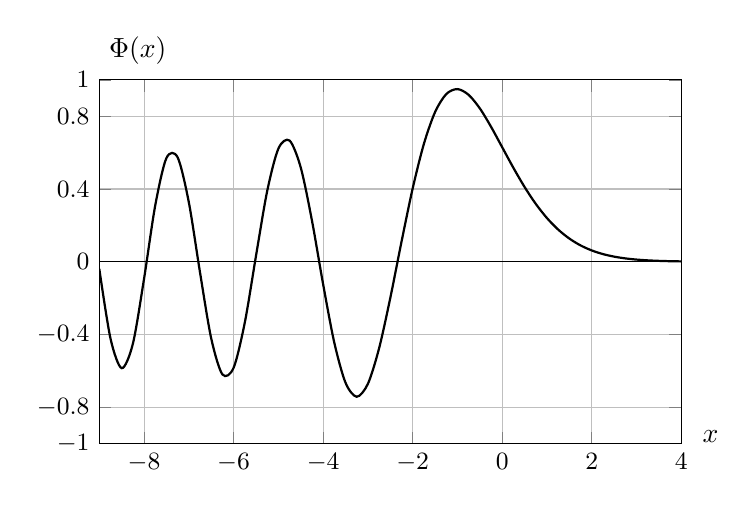
\begin{tikzpicture}
\begin{axis}[
  width=.74\linewidth,height=6.2cm,
  xmin=-9,xmax=4,ymin=-1,ymax=1,
  xtick={-8,-6,-4,-2,0,2,4},
  ytick={-1,-.8,-.4,0,.4,.8,1},
  grid=major,axis lines=box,
  xlabel={$x$},ylabel={},
  xlabel style={at={(axis description cs:1.02,.02)},anchor=west},
  ylabel style={at={(axis description cs:.04,1.02)},anchor=south},
  tick label style={font=\small},
  every axis plot/.append style={black,thick,smooth},
]
\addplot[black,thin,no marks] coordinates {(-9,0) (4,0)};
\addplot[black,thick,smooth,no marks] coordinates {
(-9.00,-0.0392) (-8.75,-0.4223) (-8.50,-0.5854) (-8.25,-0.4512)
(-8.00,-0.0934) (-7.75,0.3101) (-7.50,0.5703) (-7.25,0.5738)
(-7.00,0.3266) (-6.75,-0.0592) (-6.50,-0.4219) (-6.25,-0.6197)
(-6.00,-0.5834) (-5.75,-0.3347) (-5.50,0.0315) (-5.25,0.3882)
(-5.00,0.6217) (-4.75,0.6663) (-4.50,0.5178) (-4.25,0.2265)
(-4.00,-0.1245) (-3.75,-0.4460) (-3.50,-0.6656) (-3.25,-0.7427)
(-3.00,-0.6714) (-2.75,-0.4759) (-2.50,-0.1991) (-2.25,0.1092)
(-2.00,0.4031) (-1.75,0.6478) (-1.50,0.8229) (-1.25,0.9218)
(-1.00,0.9493) (-0.75,0.9177) (-0.50,0.8432) (-0.25,0.7422)
(0.00,0.6293) (0.25,0.5161) (0.50,0.4107) (0.75,0.3179)
(1.00,0.2398) (1.25,0.1766) (1.50,0.1272) (1.75,0.0896)
(2.00,0.0619) (2.25,0.0419) (2.50,0.0279) (2.75,0.0182)
(3.00,0.0117) (3.25,0.0074) (3.50,0.0046) (3.75,0.0028)
(4.00,0.0017)
};
\end{axis}
\node[anchor=south west] at ([yshift=2pt]current axis.north west) {$\Phi(x)$};
\end{tikzpicture}
\caption{ }\label{fig:55}
\end{figure}

Figure~55 shows the graph of the Airy function.
